\begin{center}
	{\Large\bf 第一章\;学前自测}
	
	{\it 注:加*号的题目可选作,其他均与本课程后续内容相关,为必须掌握}
\end{center}

\begin{enumerate}
%   \setlength{\itemindent}{1cm}
  \item 请在图上标出常用的三角函数值:$\sin\theta,\;\cos\theta,\;\tan\theta,\;
  \sec\theta,\;\csc\theta.$
%   \begin{center}
% 	\resizebox{!}{3.5cm}{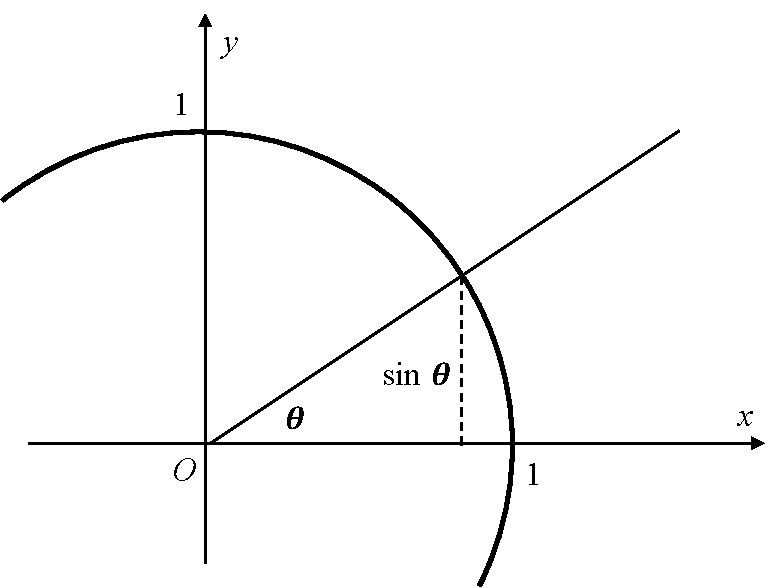
\includegraphics{./images/ch1/triFuncs.pdf}}
%   \end{center}
  \begin{figure}[!htb]
  	\centering
  	\resizebox{!}{3.5cm}{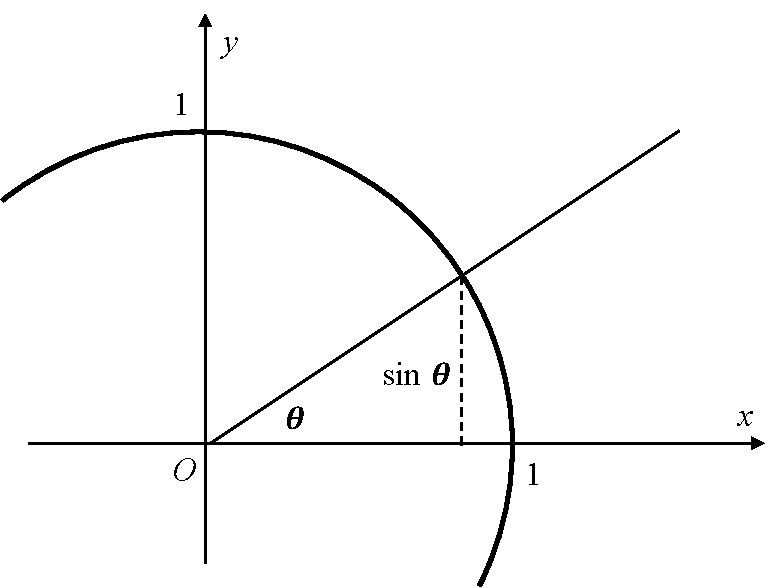
\includegraphics{./images/ch1/triFuncs.pdf}}
  \end{figure}
  \item 写出三角函数的{\it 和差化积}、{\it 积化和差}、{\it 半(倍)角公式}、{\it 万能公式}
  \item* 化简如下表达式:设$\theta\in\left(0,\pi/2\right)$
  \begin{enumerate}[(1)]
%     \setlength{\itemindent}{1cm}
    \item $\prod\limits_{i=1}^n\cos\df{\theta}{2^i}$
    \hspace{2cm}
    {\it(注:$\prod\limits_{i=1}^nf(i)=f(1)\cdot f(2)\cdot\cdots\cdot
    f(n)$)}
    \item $\sum\limits_{i=1}^n\cos i\theta$
  \end{enumerate}
  \item 证明以下等式与恒等式
  \begin{enumerate}[(1)]
    \item $\df{\pi}4=3\arctan\df14+\arctan\df5{99}$
    \item $3\arccos x-\arccos(3x-4x^3)=\pi,\;\left(|x|\leq\df12\right)$
    \item $2\arctan x+\arcsin\df{2x}{1+x^2}=\pi,\;(x>1)$
  \end{enumerate}
  \item 平面上任一点的位置可以既可以用直角坐标$(x,y)$表示,也可以用极坐标$(\rho,\theta)$
  表示,前者可用后者表示如下
  $$x(\rho,\theta)=\rho\cos\theta,\quad y(\rho,\theta)=\rho\sin\theta,$$
  反之,后者用前者应表示为(假设:$\rho\geq 0,\theta\in[0,2\pi]$)
  $$\rho(x,y)=\underline{\hspace{5cm}},\quad
  \theta(x,y)=\underline{\hspace{5cm}}.$$
  \item 比较以下函数值的大小,简述理由
  \begin{enumerate}[(1)]
    \item $x,\quad e^x-1,\quad \ln(x+1)$\quad$(x>0)$
    \item $\sin x,\quad \tan x, \quad \sec x, \quad x$ \quad $(x\in(0,\pi))$
  \end{enumerate}
  \item 证明函数$y=x+\sin x$在定义域内严格单调递增。({\it 注:函数$y=f(x)$严格单调
  递增,当且仅当对任意$x_1<x_2$,总有$f(x_1)<f(x_2)$})
  \item 本章习题中有如下定理:{\bf 任何一个定义在对称区间上的函数均可写成一个奇函数和一个
  偶函数的和},由此,
  $$e^x=\underline{\hspace{3cm}}_{\mbox{(奇)}}
  +\underline{\hspace{3cm}}_{\mbox{(偶)}}$$
  \item 写出下列集合之间的一一映射
  \begin{enumerate}[(1)]
    \item $(-1,1)\mapsto\mathbb{R}$\hspace{2cm}({\it 注:
  $\mathbb{R}=(-\infty,+\infty)$})
    \item $(0,+\infty)\mapsto\mathbb{R}$
    \item* $\{(x,y)\in\mathbb{R}^2|x^2+y^2<1\}\mapsto\mathbb{R}^2$
    \hspace{2cm}({\it 注:$\mathbb{R}^2$表示全平面)}
    \item 整数集$\mapsto$正整数集
    \item* 正整数集$\mapsto$正有理数集
  \end{enumerate}
  \item Fibnacci数列定义如下:$a_0=1$,$a_1=1$,
  $$a_{n+2}=a_{n+1}+a_{n},\quad n=1,2,\ldots,$$
  \begin{enumerate}[(1)]
    \item 请推导$\{a_n\}$的通项表达式;
    \item 设$p,q\in\mathbb{R}$,将前述递推式改为:
    $$a_{n+2}=p\cdot a_{n+1}+q\cdot a_{n},\quad n=1,2,\ldots,$$
    试讨论$\{a_n\}$通项表达式有何变化。
  \end{enumerate}
  \item* 写出不少于五位你听说过的数学家的名字(最好用英文),简述他们的事迹。
  \item 公理(Axiom)、假设(Assumption)、定理(Theorem)、定律(Law)有何异同?
  \item 以下函数中哪些是相同的,若不同,有何区别?
  $$x,\quad |x|,\quad e^{\ln x},\quad \ln(e^x),\quad \sqrt{x^2},\quad
	\frac{x^2-4}{x-2}-2,\quad
  \sin(\arcsin x),\quad \arcsin(\sin x), \quad \tan(\arctan x)$$
  \item 取整函数$[x]$的定义为{\it 不大于$x$的最大整数},请利用取整函数给出以下曲线的方程:
  \begin{center}
	\resizebox{!}{2.5cm}{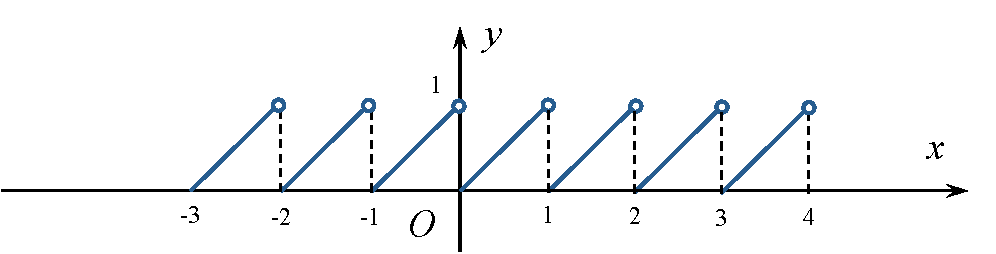
\includegraphics{./images/ch1/f1.pdf}}\\
	\resizebox{!}{2.5cm}{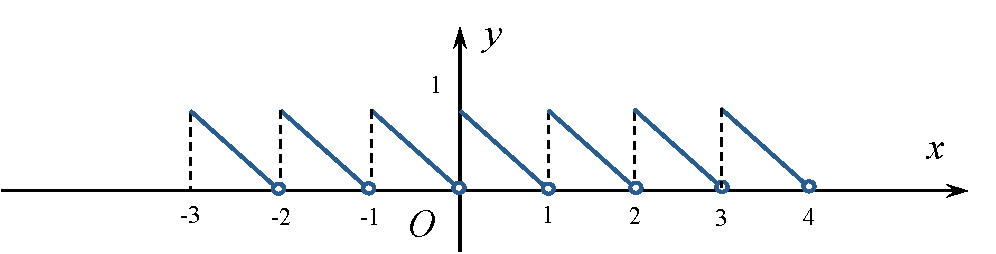
\includegraphics{./images/ch1/f2.pdf}}\\
	\resizebox{!}{2.5cm}{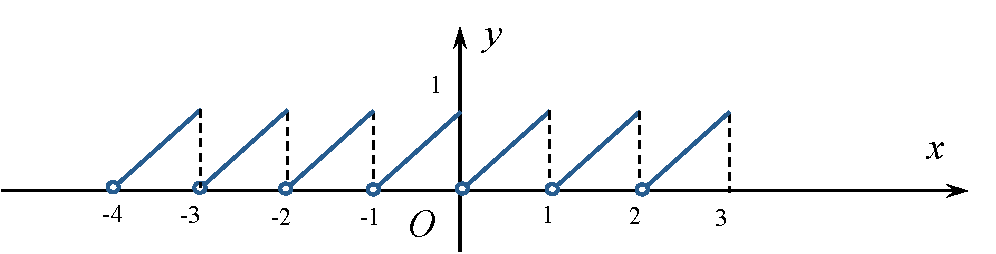
\includegraphics{./images/ch1/f3.pdf}}
  \end{center}
  \item 设$a\in\mathbb{R}$,且对任意$x\in\mathbb{R}$,有
  $f(2a-x)=f(x)$,
  请问$y=f(x)$的图像具有怎样的几何性质?若上式改为$f(2a-x)=-f(x)$,对应几何性质有何改变?
  \item 设$a\in\mathbb{R}$,且对任意$x\in\mathbb{R}$,有
  $f(a-x)=g(x)$,请问$y=f(x)$和$y=g(x)$的图像有何关系?
  \item 若对任意$x_1,x_2$,总有
  $[f(x_1)-f(x_2)](x_1-x_2)\leq 0$,
  由此可知函数$y=f(x)$具有何种性质?
  \item 给定集合$A\subset\mathbb{R}$,若$A$有界,是否必有最大和最小值?
  是否必有{\it 上确界}(最小的上界)和{\it 下确界}(最大的下界)?
  若$A$无界,是否必为无穷集合?
\end{enumerate}